\chapter{Discussion}
\label{chap:discussion}

With the disks now fit, we may interpret our results. Since this project was based around the question of how environment influences protoplanetary disks, we would like to compare our best fit values to other disks, including to one other from the ONC \citep{Factor2017} as well as to others outside of it. We also consider how our results compare to modeling efforts.


\section{Reflections on the Fits}

Looking at the fits to our three molecular lines side by side, several things jump out. First and foremost, as discussed in \S\ref{subsection:co_fit}, our attempts to fit the CO line were overwhelmed by the significant cloud contamination around the disk. If this run had converged, we would have used its disk mass results in the other runs, but since these results are not to be trusted, we instead continued to use the disks' mass values presented in \citet{Williams2014}, which were inferred from continuum emission.


The \hco and HCN runs converged into impressive agreement, although their posteriors show that \hco line resulted in a much more confident model. Both lines show surprisingly high chemical abundances in disk A, while both also show significantly lower values for disk B abundances (discussed below). The two lines' fits for disk A's outer radius agree to within around 1\% (although the HCN fit is significantly less certain than the \hco fit) and the lines' best-fit $q$ values agree to within 15\%. Atmospheric temperatures for disk A in both lines are large and significantly different, with the \hco line preferring a temperature 50\% greater than HCN's, but this is at least somewhat expected, as the two molecules are emitting from different regions of the disk and thus could reflect different regions of its temperature profile. In both lines, disk A's temperature structure power law index, $q$, is decidedly positive, although we expect this parameter to not settle with absolute certainty on a single value, since the observations don't have enough spatial resolution to constrain it tightly.

Fits for disk B are systematically less well constrained, since it is smaller, unresolved, and more easily overrun by excess emission from disk A and cloud contamination. Still, save for the disk's outer radius fit, all parameters are generally within the range of expected values.

As discussed in \S\ref{subsection:hcn_fit}, a posteriori cuts of the HCN model's MCMC chain limiting disk B's outer radius to $\geq$220 AU changes the best-fit parameters significantly, most notably leading the fits of disk B's outer radius in \hco and HCN into agreement and pushing disk A's HCN abundance more than a full order of magnitude higher, and into nearly perfect agreement with results from HCN fitting in \citet{Factor2017}. Whether this is a reasonable thing to do is not clear to me.

We see in the HCN channel maps an area of significant flux coming from between disks around $ v = 10.24-9.83$. This may be region where the two disks are interacting, a possibility that our model does not take into account. The feature is less clearly present in \hco and invisible in CO, likely overrun by cloud contamination.


That each disk's abundances are so different from one another is something of a surprise. Both disks have fairly similar ratios of the two emitting molecules: disk A's \hco/HCN ratio of log abundances is 1.09, while disk B's is 0.95\footnote{These ratios become 1.21 for disk A and unity for disk B if the disk B radius cut is made.}. \citet{Williams2014} posit that wide binaries (systems with separations $\geq$ 300 au), such as this one, do not form in the same initial cloud structures\footnote{Jonathan doesn't actually put any references on this; I have no idea where he got it from. He just puts in references to other papers looking at misaligned binaries}. If this is the case, the notable differences in abundances between disk A and disk B could indicate that the disks in d253-1536 formed separately in clouds with different chemical compositions before joining together later. This is, of course, entirely speculative, but is a possibility.




\section{Comparison with the Literature}

We would now like to contextualize our results in the context of the larger field of protoplanetary disk studies.


\subsection{Line Emission Modeling}


\begin{table}[ht!]
  \centering
  \begin{threeparttable}
    \caption{Disk Parameter List}
    \label{table:comparisons}
    \renewcommand{\arraystretch}{1.2}
    \begin{tabular}{l l l c c c }
      \toprule \toprule
      %\multirow{2}{*}{Parameter} & \multirow{2}{*}{Disk A}    & \multicolumn{2}{c}{Disk B} \\
      Reference                             & Source     & Line          & $q$ & log X$_\text{mol}$ & Atms. Temp\\
      \midrule %\midrule
      \multirow{3}{*}{This study}           & d253-1536a & \hco(4-3)      & $0.66$  & $-7.96$         & $151$  \\
                                            & d253-1536a & HCN(4-3)       & $0.72$  & $-7.62$         & 140  \\
                                            & d253-1536a & CO(3-2)\tnote{a} & $0.40$  & $[-4]$        & 1  \\
      \hline
      \multirow{3}{*}{\cite{Factor2017}}   & d216-0939  & \hco(4-3)      & $0.17$  & $-10.08$        & 190  \\
                                           & d216-0939  & CO(3-2)        & $-0.33$ & $[-4]$          & 70  \\
                                           & d216-0939  & HCN(4-3)       & $-0.18$ & $-6.7$          & 19  \\
      \hline
      \multirow{2}{*}{\citet{Flaherty2015}}& HD163296   & CO(3-2)        & $-0.22$ & $[-4]$          & 94  \\
                                           & HD163296   & CO(2-1)        & $-0.27$ & $[-4]$          & 79  \\
      \hline
      \citet{Hughes2008}\tnote{b}           & A bunch    & CO(3-2)        &  -    & $[-4]$          & -  \\
      \hline
      \citet{Rosenfeld2012}\tnote{b}        & V4046 Sgr  & $^{12}$CO(2-1) & $-0.63$ & $[-4]$           & -  \\
      \hline
      \citet{Flaherty2017}\tnote{c}         & HD163296   & DCO$^+$(3-2)   & $[-2.22]$ & $-10.79$      & [94]  \\
      \hline
      \citet{Zhang2017}                     & TW Hya     & $^{13}$C$^{18}$O(3-2), C$^{18}$O(3-2)  & $-0.47$ & -7.96 & 151  \\
      \hline
      \citet{Flaherty2018}\tnote{d}         & TW Hya     & CO(6-5, 3-2, 2-1) & $-0.46$ & $[-4]$       & 31  \\
      \bottomrule
    \end{tabular}
    \begin{tablenotes}\footnotesize
      \item[*] Values in [brackets] were fixed during fitting.
      \item[\dagger] Since there is not a convention about whether a negative value of $q$ indicates a radially decreasing or increasing temperature structure (in other words, whether or not $q$ is implicitly negative), some of these values have the opposite sign of the value reported in their article. When this is the case, it indicates that, in that original paper, atmospheric temperature was defined such that T$_{atms} \propto r^{-q}$. In our work, and in all the values given here, it is the case that T$_{atms} \propto r^{q}$, meaning that a negative value of $q$ leads to temperature decreasing with radius.
      \item[a] This result is being presented for completeness (and to allow for the chance that something changes dramatically in coming runs REWORK), but since its T$_{atms}$ clearly got stuck, it is not a useful result for comparison and will not be discussed.
      \item[b] \cite{Rosenfeld2012} didn't fit for tatms
      \item[c] In \citet{Flaherty2017}, they fit three rings, and consequently have three slightly different values for each parameter. The values reported here are for their middle ring, although the three do not vary significantly from one another. Additionally, T$_{atms}$ and $q$ were fixed at values found for CO(3-2) in \citet{Flaherty2015}, and only X$_\text{mol}$ was fit for.
      \item[d] \citet{Flaherty2018} developed several models, with different morphological structures. The results presented here are drawn from their simplest (fiducial) model.
    \end{tablenotes}
  \end{threeparttable}
\end{table}

In Table \ref{table:comparisons} we compare our results to those from other studies that have modeled line emission from protoplanetary disks. The most immediately relevant of these is the work by \citet{Factor2017}, in which they use a similar modeling technique to characterize another ONC proplyd from the same survey as our binary, and thus represents the only other disk studied in this way that is also in a high-mass star forming region. The others are well-studied disks in low-mass regions. We may compare our temperature profiles and abundance to these other systems and look for variations from expected values.

Comparing our results for disk A to these other studies, we can see that our atmospheric temperatures in \hco(4-3) and HCN(4-3) are consistent with the results of the \hco fit in \citet{Factor2017}. They are, however, significantly higher than any other study's fit.

% The slightly positive value of q derived for HCO+ is most likely due to the effect of observing an optically thin line of a molecule that freezes out in the midplane. As Schwarz et al. (2016) explain in a similar investigation of the molecular line emission from the disk around TW Hya, a flat temperature profile is expected in the case where most of the detected emission originates from the layer of the disk just above the freeze-out temperature.


Additionally, our temperature structures for both \hco and HCN are solidly positive, reflecting a temperature structure that increases with radius. As with the atmospheric temperature, this is contrasted by all other results, which have moderately negative values, save again for that of the \citet{Factor2017} \hco line, which is also positive but less so than in our fits. Our positive values stand somewhat in contrast to the $q$ value of $-0.5_{-0.1}^{0.2}$ predicted by \citet{Dartois2003} for a geometrically flat, optically thin disk.


% It is (seems?) possible that these discrepancies in $q$ and X$_{mol}$ could reflect the fact that our fits had different values for some of the fixed parameters. These include R$_{crit}$, which we fix at 100 and Sam fixed at 600 AU, as well as $z_q$ and $T_\text{mid}$\footnote{Since Sam fit multiple lines simultaneously, they were able to constrain these parameters, which is not possible in the case of single-line fitting.}, which they fit for by simultaneously fitting CO and \hco emission and yielding values of $z_{q, 150} = 73$ AU and T$_{mid} = 24.7$ K, in comparison to our values of 29 and 19, respectively.


Our molecular abundances for each disk vary from those reported in the \citet{Factor2017} paper, the only other study to model \hco emission. In it, they report finding canonical values for the \hco line (log X$_{\hco}$ = $-10.04$) and unexpectedly high values for the HCN line (log X$_{HCN}$ = $-6.7$), contrasted by our findings of $-8.36$ and $-7.62$, respectively\footnote{Although, as described above, removing samples with large outer radii for disk B pushes disk A's HCN abundance to -6.98, within the uncertainties of their HCN fit.}.


We may also compare these abundances to theoretical modeling efforts. \citet{Walsh2010} developed radial and vertical chemical models for an imaginary isolated protoplanetary disk around a T-Tauri star (a system similar to the famous TW Hya), studying molecular abundance distributions throughout the disk for molecules within ALMA's reach. They showed that log abundances in their models for \hco varied from $-8$ to $-12$, $-7$ to $-12$ for HCN, and $-4$ to $-9$ for CO. The authors then built on this model by adding robust modeling of externally-driven UV and X-ray ionization \citep{Walsh2012} and applying it to the same disk system, this time with an O star nearby providing ionizing photons \citep{Walsh2013}. They then make the same molecular abundance distribution maps as before (see Fig. \ref{fig:walsh-abundance-profs}). The authors note that, in their model photoionized disk, \hco column density increases by a factor of 6.3 relative to the isolated disk, whereas HCN and CO column densities remain constant through ionization\footnote{This would be useful if we had an estimation of what the \hco/HCN ratio would be in these two disks. They do have column density ratios in Walsh13; is it reasonable to say (I guess it would have to be in the case of optically thin emission) that col dens $\propto$ abundance? If that were the case then we'd be golden.}. They also note that the ionized disks have much higher gas temperatures, $\gg$ 50 K, which is consistent with our findings.


Although our modeling assumes a constant chemical abundance across the whole disk, these models offer a way to confirm that our results are within the predicted ranges, despite the fact that the \hco abundance is significantly higher than the values found by other studies.



\begin{figure}[t]
  \hspace*{\fill}%
  \subcaptionbox{CO abundances}{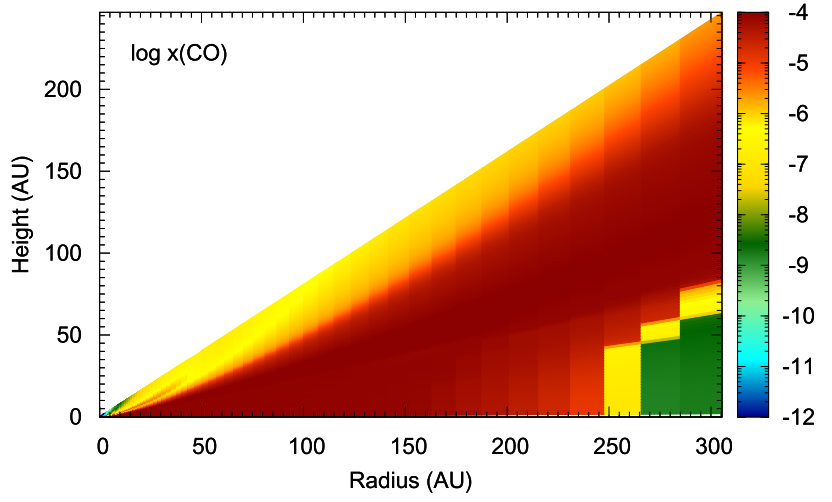
\includegraphics[width=0.33\linewidth]{walsh10_Xco.png}}%
  \subcaptionbox{\hco abundances}{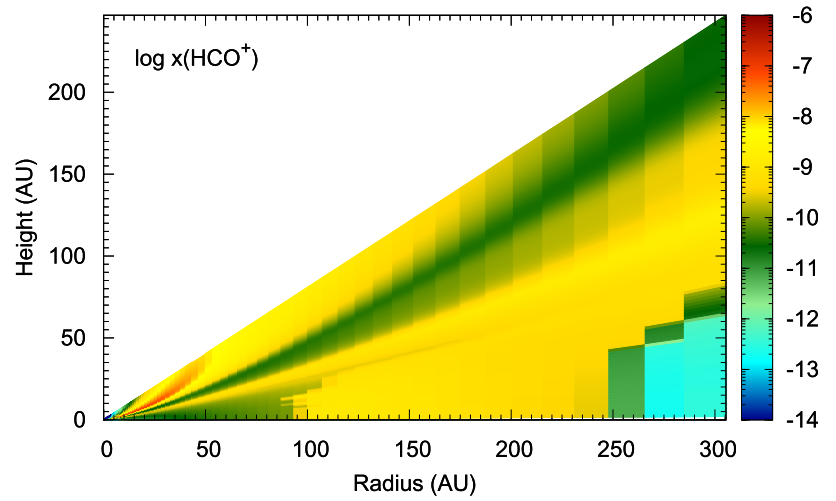
\includegraphics[width=0.33\linewidth]{walsh10_Xhco.png}}%
  \subcaptionbox{HCN abundances}{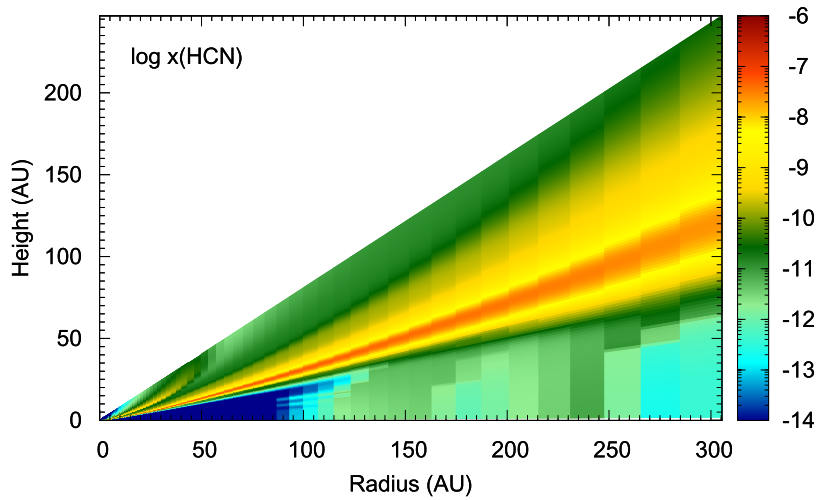
\includegraphics[width=0.33\linewidth]{walsh10_Xhcn.png}}\vfill%
  \subcaptionbox{CO abundances}{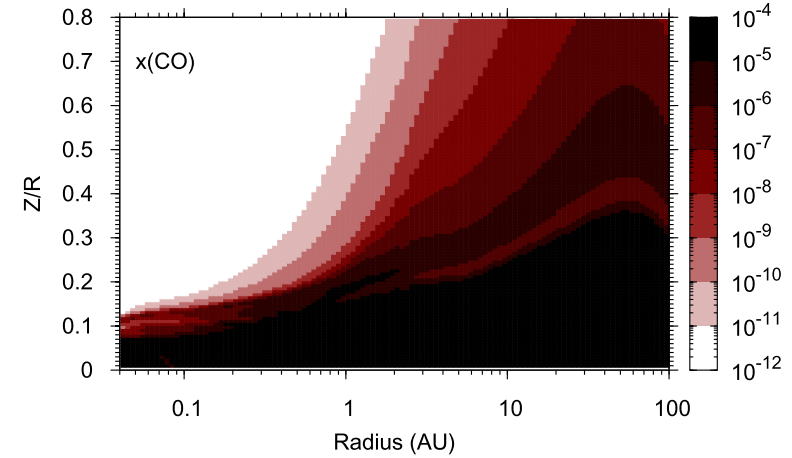
\includegraphics[width=0.33\linewidth]{walsh13_Xco.png}}%
  \subcaptionbox{\hco abundances}{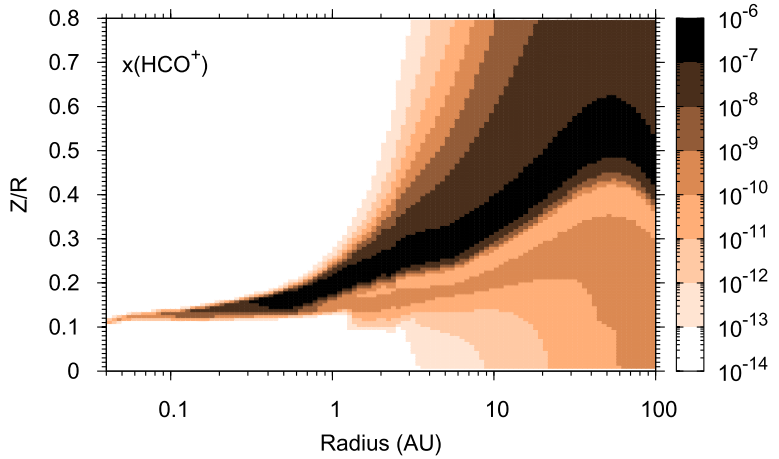
\includegraphics[width=0.33\linewidth]{walsh13_Xhco.png}}%
  \subcaptionbox{HCN abundances}{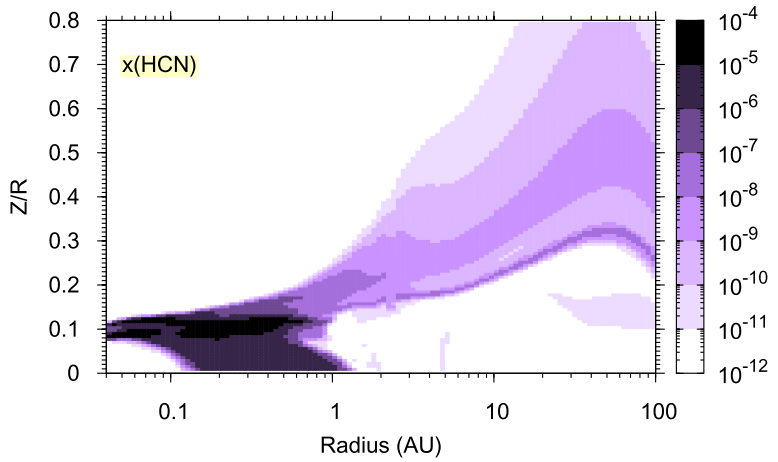
\includegraphics[width=0.33\linewidth]{walsh13_Xhcn.png}}%
  \hspace*{\fill}%
  \caption{Models showing radial and vertical distributions of CO, \hco, and HCN in a simulated disk around a T-Tauri star. The top row shows the profiles of isolated disks \citep{Walsh2010}, while the bottom row shows the profiles of disks being irradiated by a nearby O star \citep{Walsh2013}. Note that bottom row is on a log scale and only covers the inner 100 AU of the disk, while the top row is linearly scaled and shows a 300AU stretch. \textit{It seems like only having one of these sets of images would make more sense.}}
  \label{fig:walsh-abundance-profs}
\end{figure}




\subsection{Population Comparison}

We can also compare our disks' mass and radius to other protoplanetary disks. While these features may provide less nuanced insight, they are more easily measured, giving us a broader sample of disks to compare ours to. For these comparisons, we again draw on the disks' inferred gas mass measurements made by \citet{Williams2014}, which carry with them significant uncertainty on account of the 100:1 assumed gas:dust ratio (as described in \S\ref{chap:introduction}). As such, the values we use for the masses of disk A and disk B are 0.075 M$_\odot$ and 0.029 M$_\odot$ (78.66 and 29.88 Jovian masses), respectively. Our best-fit values for radii from the MCMC models were around 337 and 145 AU, respectively.

In the survey that originally provided these data, \citet{Mann2014} provided initial disk masses, as well as semi-minor and -major axes of the disks, approximate measures of the disks' radial extents. Disk A in the present system was, by their measure, the most massive disk in the study, 75\% more massive than the study's next most massive disk, d216-0939 (which was the subject of \citet{Factor2017}); disk B was the fifth most massive. Disk A had the study's fourth largest semi-major axis\footnote{The authors' measurement of disk A's semi-major axis, at 268 au, is 20\% smaller than our fit measurements. The survey's reported semi-major axis for d216-0939 was also smaller than the fit value in \citet{Factor2017}, though by only 6\%.}. The authors did not fit disk B's radial extent; however, our measurement of 145 AU would make it the eleventh (out of 22) largest disk in the survey. Thus, disk A is on the very high end of the study's mass and radius range, while disk B is apparently quite dense and of median radial extent.


In \citet{Miotello2016}, the authors analyze several CO isotopologues to retrieve the gas masses of 34 protoplanetary disks in Lupus. In it, they report surprisingly low masses, reflective of their calculated gas/dust ratios, which systematically fall well below the traditional value of 100. Their resulting gas masses are far smaller than those found by \cite{Mann2014} in the ONC; here, most of the survey's masses are between $10^{-5}$ to $10^{-3}$ M$_\odot$, with the most massive at 1.5 $\times 10^{-3}$ M$_\odot$ (1.6 Jovian masses). since the disks were not spatially resolved, radii were not measured.


\citet{Ansdell2016} and \citet{Ansdell2018} characterized the mass (both dust and gas) and radius distributions of protoplanetary disks in Lupus using CO isotopologues and continuum emission. To derive gas masses, they assumed a CO/H$_2$ ratio of $10^{-4}$ and then used the isotopologues' ratios to find total masses. Of these gas masses that they were able to constrain, they found disks to range from around 1-10 Jovian masses.


\citet{Eisner2018} conducted a particularly comprehensive survey of disks in $\sigma$ Ori, a young cluster in the ONC, north of M42 and M43. In their survey, they trace dust masses, so maybe it's not terribly useful. Still, they note that disks in their survey are particularly compact.

\begin{figure}[h!]
  \centering
    \hspace*{\fill}%
    \subcaptionbox{\hco}{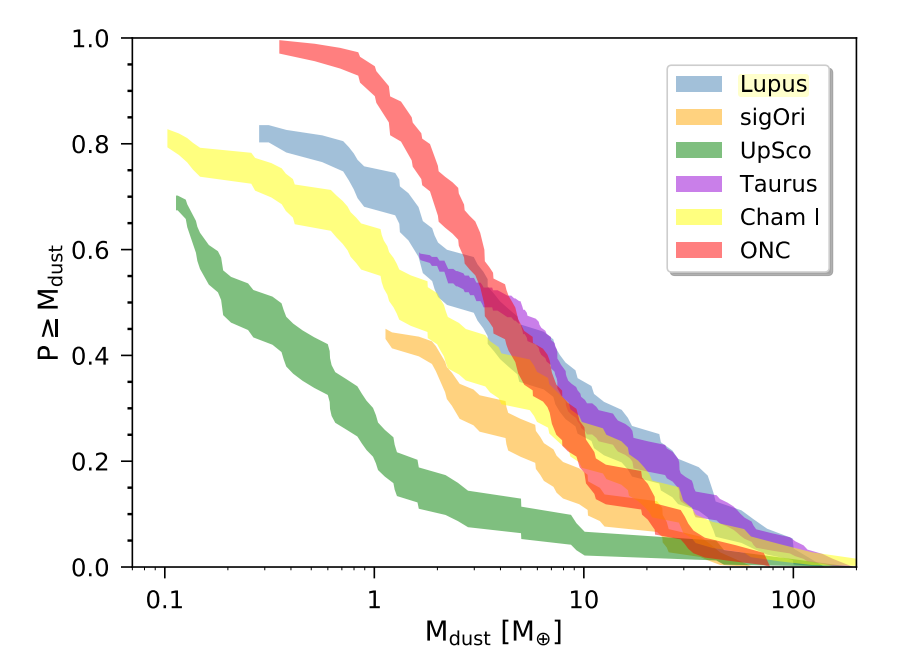
\includegraphics[width=0.5\linewidth]{dust_mass_dist_Eisner18.png}}%
    \subcaptionbox{HCN}{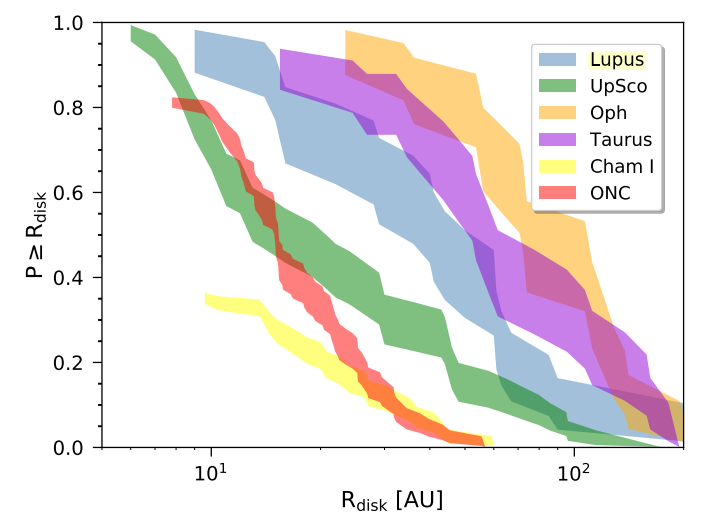
\includegraphics[width=0.5\linewidth]{dust_radius_dist_Eisner18.png}}%
    \hspace*{\fill}%
    \caption{Some stuff from Eisner2018.}
    \label{fig:bf_disk_strs}
\end{figure}

% \citet{Cieza2019} also has stuff for this

I don't really know what else to say here. Seems like ours are big, dense disks. Would be really nice to calculate that gas mass on my own.



\section{Remarks}
These disks appear to be somewhat atypically large and dense. They may have formed separately. More work should be done. Etc





\textit{This section still feels a little incomplete; I don't really know what else to do with it. Would love to hear your thoughts/guidance.}


% Kamp overview:
% https://arxiv.org/pdf/1901.10862.pdf




% No density profile == No MMSN bs
% \section{Planet-Forming Potential}
% \label{section:fitting_procedure}
%
%
% One way to contextualize the results presented in \S\ref{chap:analysis} is through the lens of planet formation. This analysis traditionally begins with a comparison to the MMSN, which is the density profile that our own Solar System would have if all our planets had gas added to them until their composition matched that of the Sun, then each planet's mass was spread out in a ring along its orbital path (as discussed in \S\ref{chap:introduction}). Integrating this mass leaves us with $M_\text{MMSN} \approx 0.01 M_\odot$. It is worth reiterating that this is an extremely rough metric, build on several assumptions, and that it does not reflect \textit{minimum} mass of a planet forming potential, but rather an approximation of the mass it would take for a disk like ours to form.
%
% With the extremely large mass of $M = 0.36M_\odot$ that we measure in the CO line, it is needless to say that the disk's mass would not be its limiting factor in planet formation.











% The End
